\section{Binary Search Trees, Sets and Maps}

\begin{frame}
	\frametitle{Definition}
	A binary search tree ...
	\begin{itemize}
		\item is a tree ( :O )
		\item is binary ( :O ). So, two children maximum, that we name "left" and "right"
		\item such that each nodes stores a "key" and a "value" (which can be the same as the key)
		\item respects the "search property": 
		\begin{itemize}
			\item all nodes on the left subtree are $<$ the current node
			\item all nodes on the right subtree are $>$ the current node
		\end{itemize}
	\end{itemize}
\end{frame}

\begin{frame}
	\frametitle{Invalid BST example}
	
	\begin{center}
		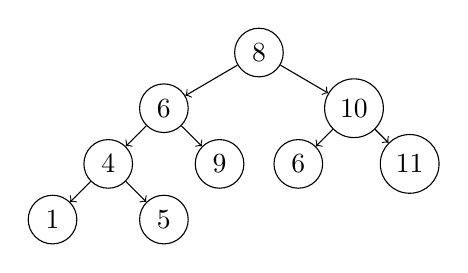
\begin{tikzpicture}[->,nodes={draw, circle}]
		\node (a8) [] {8};
		\node (a6) [below left of = a8, xshift=-0.5cm] {6};
		\node (a10) [below right of = a8, xshift=0.5cm]{10};
		\node (a4) [below left of = a6]{4};
		\node (a7) [below right of = a6]{9};
		\node (a9) [below left of = a10]{6};
		\node (a11) [below right of = a10]{11};
		\node (a1) [below left of = a4]{1};
		\node (n7) [below right of = a4]{5};
		\draw (a8) -> (a10);
		\draw (a8) -> (a6); 
		\draw (a6) -> (a4);
		\draw (a6) -> (a7);
		\draw (a10) -> (a9);
		\draw (a10) -> (a11);
		\draw (a4) -> (a1);
		\draw (a4) -> (n7);
		\end{tikzpicture}
	\end{center}
\end{frame}

\begin{frame}
	\frametitle{BST example}
	
	\begin{center}
		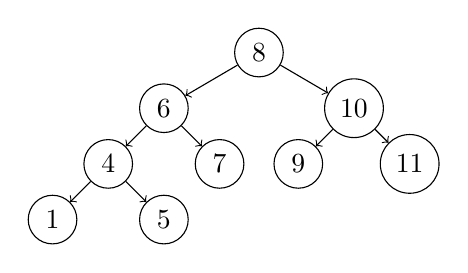
\begin{tikzpicture}[->,nodes={draw, circle}]
		\node (a8) [] {8};
		\node (a6) [below left of = a8, xshift=-0.5cm] {6};
		\node (a10) [below right of = a8, xshift=0.5cm]{10};
		\node (a4) [below left of = a6]{4};
		\node (a7) [below right of = a6]{7};
		\node (a9) [below left of = a10]{9};
		\node (a11) [below right of = a10]{11};
		\node (a1) [below left of = a4]{1};
		\node (n7) [below right of = a4]{5};
		\draw (a8) -> (a10);
		\draw (a8) -> (a6); 
		\draw (a6) -> (a4);
		\draw (a6) -> (a7);
		\draw (a10) -> (a9);
		\draw (a10) -> (a11);
		\draw (a4) -> (a1);
		\draw (a4) -> (n7);
		\end{tikzpicture}
	\end{center}
\end{frame}

\begin{frame}
	\frametitle{Balanced Search Tree}
	A (binary) tree is said to be balanced if its height is minimal, that is if its height is $\floor{\log_2(n)}$
	
	Most the of the BST are balanced. We will see later why...
        We can write BBST for \textit{Balanced Binary Search Tree}.
\end{frame}

\begin{frame}
	\frametitle{Common operations}
	\begin{itemize}
		\item search(key): returns the value associated with the key
		\item insert(key, value): insert a new key/value
		\item findMax(): returns the key/value associated with the biggest key
		\item findMin(): ...
		\item successor(key): returns the key/value immediately after the given key
		\item predecessor(key): ...
	\end{itemize}
\end{frame}

\begin{frame}
	\frametitle{Implementing search operations}
	Let's say we want to find the value associated with $5$ in this tree:
	
	\begin{center}
		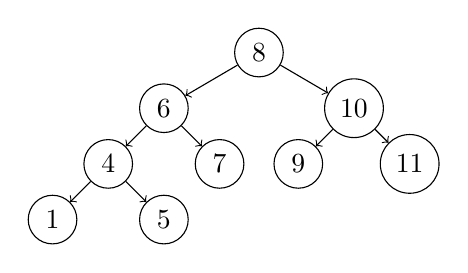
\begin{tikzpicture}[->,nodes={draw, circle}]
		\node (a8) [] {8};
		\node (a6) [below left of = a8, xshift=-0.5cm] {6};
		\node (a10) [below right of = a8, xshift=0.5cm]{10};
		\node (a4) [below left of = a6]{4};
		\node (a7) [below right of = a6]{7};
		\node (a9) [below left of = a10]{9};
		\node (a11) [below right of = a10]{11};
		\node (a1) [below left of = a4]{1};
		\node (n7) [below right of = a4]{5};
		\draw (a8) -> (a10);
		\draw (a8) -> (a6); 
		\draw (a6) -> (a4);
		\draw (a6) -> (a7);
		\draw (a10) -> (a9);
		\draw (a10) -> (a11);
		\draw (a4) -> (a1);
		\draw (a4) -> (n7);
		\end{tikzpicture}
	\end{center}
\end{frame}

\begin{frame}
	\frametitle{Implementing search operations}
	Let's start at the root:
	
	\only<2>{8 > 5: search only on the left}
	
	\begin{center}
		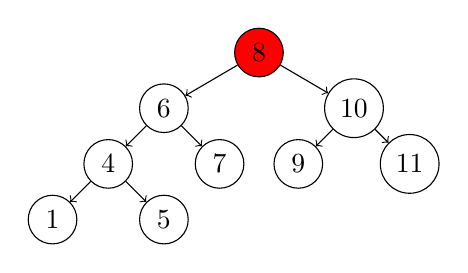
\begin{tikzpicture}[->,nodes={draw, circle}]
		\node (a8) [fill=red] {8};
		\node (a6) [below left of = a8, xshift=-0.5cm] {6};
		\node (a10) [below right of = a8, xshift=0.5cm]{10};
		\node (a4) [below left of = a6]{4};
		\node (a7) [below right of = a6]{7};
		\node (a9) [below left of = a10]{9};
		\node (a11) [below right of = a10]{11};
		\node (a1) [below left of = a4]{1};
		\node (n7) [below right of = a4]{5};
		\draw (a8) -> (a10);
		\draw (a8) -> (a6); 
		\draw (a6) -> (a4);
		\draw (a6) -> (a7);
		\draw (a10) -> (a9);
		\draw (a10) -> (a11);
		\draw (a4) -> (a1);
		\draw (a4) -> (n7);
		\end{tikzpicture}
	\end{center}
\end{frame}

\begin{frame}
	\frametitle{Implementing search operations}
	We are now at 6
	
	\only<2>{6 > 5: search only on the left}
	
	\begin{center}
		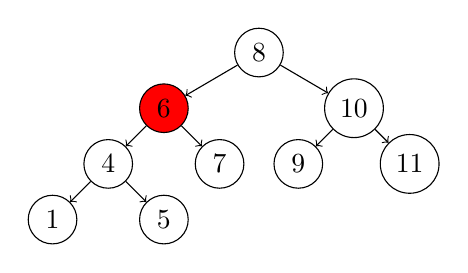
\begin{tikzpicture}[->,nodes={draw, circle}]
		\node (a8) [] {8};
		\node (a6) [below left of = a8, xshift=-0.5cm, fill=red] {6};
		\node (a10) [below right of = a8, xshift=0.5cm]{10};
		\node (a4) [below left of = a6]{4};
		\node (a7) [below right of = a6]{7};
		\node (a9) [below left of = a10]{9};
		\node (a11) [below right of = a10]{11};
		\node (a1) [below left of = a4]{1};
		\node (n7) [below right of = a4]{5};
		\draw (a8) -> (a10);
		\draw (a8) -> (a6); 
		\draw (a6) -> (a4);
		\draw (a6) -> (a7);
		\draw (a10) -> (a9);
		\draw (a10) -> (a11);
		\draw (a4) -> (a1);
		\draw (a4) -> (n7);
		\end{tikzpicture}
	\end{center}
\end{frame}

\begin{frame}
	\frametitle{Implementing search operations}
	We are now at 4
	
	\only<2>{4 < 5: search only on the right}
	
	\begin{center}
		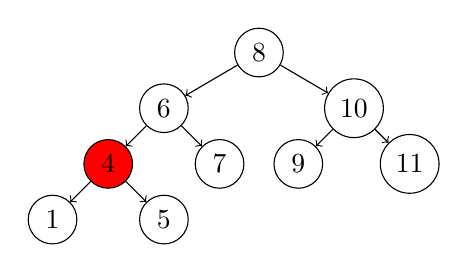
\begin{tikzpicture}[->,nodes={draw, circle}]
		\node (a8) [] {8};
		\node (a6) [below left of = a8, xshift=-0.5cm] {6};
		\node (a10) [below right of = a8, xshift=0.5cm]{10};
		\node (a4) [below left of = a6, fill=red]{4};
		\node (a7) [below right of = a6]{7};
		\node (a9) [below left of = a10]{9};
		\node (a11) [below right of = a10]{11};
		\node (a1) [below left of = a4]{1};
		\node (n7) [below right of = a4]{5};
		\draw (a8) -> (a10);
		\draw (a8) -> (a6); 
		\draw (a6) -> (a4);
		\draw (a6) -> (a7);
		\draw (a10) -> (a9);
		\draw (a10) -> (a11);
		\draw (a4) -> (a1);
		\draw (a4) -> (n7);
		\end{tikzpicture}
	\end{center}
\end{frame}

\begin{frame}
	\frametitle{Implementing search operations}
	We are now at 5. Return the key/value pair.
	
	\begin{center}
		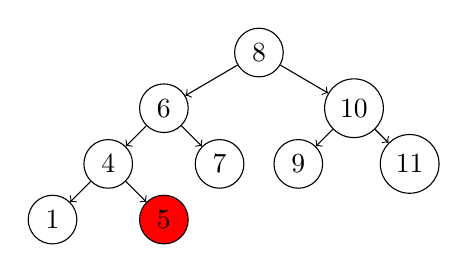
\begin{tikzpicture}[->,nodes={draw, circle}]
		\node (a8) [] {8};
		\node (a6) [below left of = a8, xshift=-0.5cm] {6};
		\node (a10) [below right of = a8, xshift=0.5cm]{10};
		\node (a4) [below left of = a6]{4};
		\node (a7) [below right of = a6]{7};
		\node (a9) [below left of = a10]{9};
		\node (a11) [below right of = a10]{11};
		\node (a1) [below left of = a4]{1};
		\node (n7) [below right of = a4, fill=red]{5};
		\draw (a8) -> (a10);
		\draw (a8) -> (a6); 
		\draw (a6) -> (a4);
		\draw (a6) -> (a7);
		\draw (a10) -> (a9);
		\draw (a10) -> (a11);
		\draw (a4) -> (a1);
		\draw (a4) -> (n7);
		\end{tikzpicture}
	\end{center}
\end{frame}

\begin{frame}
	\frametitle{Complexity?}
	$O(\text{height of the tree})$
	$= O(\floor{\log(n)})$ if the tree is balanced
	\vspace{2cm}
	Without a balanced tree, all the operations are $O(n)$!
\end{frame}

\begin{frame}
	\frametitle{Implementing a BBST}
	Ideas?
\end{frame}

\begin{frame}
	\frametitle{Implementing a BBST}
	\begin{figure}
		\centering
		\includegraphics[width=0.7\linewidth]{toohard}
	\end{figure}
\end{frame}

\begin{frame}
	\frametitle{Implementing a BBST}
	\begin{itemize}   
		\item Actually, it's not so hard
                \item But it's not always necessary
		\item We will see that in another lesson
	\end{itemize}
	BBSTs can support a lot of other (more advanced) operations, but for the operations described above, we don't need to implement a BBST. We can just use an existing one.
\end{frame}

\begin{frame}
	\frametitle{Use the STL}
	(real) languages come with implementations of BBSTs, in two categories
	\begin{itemize}
		\item Set: represents a mathematical set. It is, in fact, a BST with keys==values
			\begin{itemize}
				\item C++: std::set
				\item Java: TreeSet
			\end{itemize}
		\item Map: dictionary
		\begin{itemize}
			\item C++: std::map
			\item Java: TreeMap
		\end{itemize}
	\end{itemize}
\end{frame}